\begin{surferPage}[7-угольник]{Семиугольная симметричная септика}
Это - поверхность седьмого порядка, похожая на рождественскую звезду. До последнего времени она представляла собой септику с максимально известным количеством действительных точек сингулярности ($84$). В 2004 году этот «рекорд» был улучшен Оливером Лабсом, теперь максимальное количество таких точек – $99$.  
  
Три подушечки, находящиеся у семиугольной симметричной септики (большое изображение) друг над другом, порождаются, как и в случае с октикой Чмутова (предыдущая поверхность), благодаря использованию многочленов Чебышёва. Поэтому не удивительно, что и эта поверхность является одним из вариантов поверхностей Чмутова. Здесь плоскую кривую $T_d(x)+T_d(y)$ заменяет правильный семиугольник
    $S_7(x,y)$: 
   \[S_7(x,y) + \lambda \cdot T_d(z) = 0,\lambda\in\RR.\]
    \vspace*{-1.75em}
    \begin{center}
      \begin{tabular}{c@{\qquad}c}
        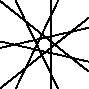
\includegraphics[height=1.5cm]{./../../common/images/labsseptic1.pdf}
        &
        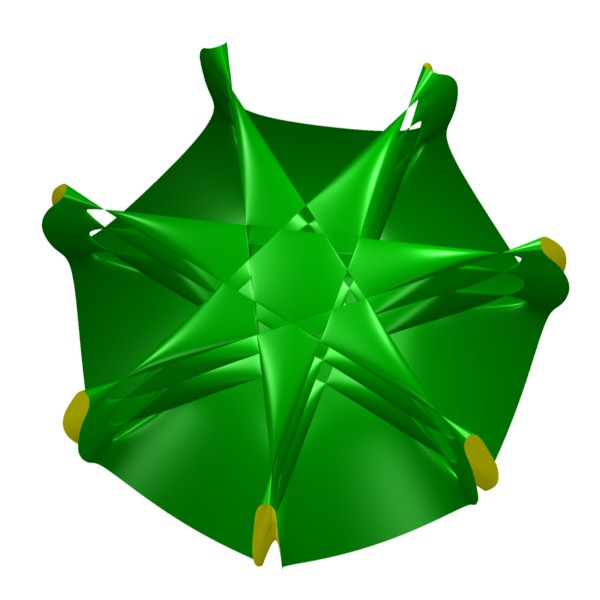
\includegraphics[height=1.5cm]{./../../common/images/septic_7eck_von_oben}
      \end{tabular}
    \end{center}
    \vspace*{-0.3em}   
	Этот вариант конструкции Чмутова разработан Дуко ван Cтратеном.
\end{surferPage}
